\documentclass[12pt, letterpaper]{article}
\usepackage{graphicx} % Required for inserting images
\graphicspath{{./figures/}}
\usepackage{listings} % Required for inserting code
\usepackage{xcolor} % Required for formatting code

\title{Assignment 1 - LaTeX Write Up}
\author{Connor Fleischman}
\date{October 3, 2024}

\definecolor{codegreen}{rgb}{0,0.6,0}
\definecolor{codegray}{rgb}{0.5,0.5,0.5}
\definecolor{codepurple}{rgb}{0.58,0,0.82}
\definecolor{backcolour}{rgb}{0.95,0.95,0.92}

\lstdefinestyle{mystyle}{
   backgroundcolor=\color{backcolour},   
   commentstyle=\color{codegreen},
   keywordstyle=\color{magenta},
   numberstyle=\tiny\color{codegray},
   stringstyle=\color{codepurple},
   basicstyle=\ttfamily\footnotesize,
   breakatwhitespace=false,         
   breaklines=true,                 
   captionpos=b,                    
   keepspaces=true,                 
   numbers=left,                    
   numbersep=5pt,                  
   showspaces=false,                
   showstringspaces=false,
   showtabs=false,                  
   tabsize=2
}

\lstset{style=mystyle}


\begin{document}
\maketitle

\section{Assignment Results} \label{AssignmentResult}
After implementing each part of Assignment 1 and testing each piece to ensure its functioning properly, here are the results.
\begin{center}
   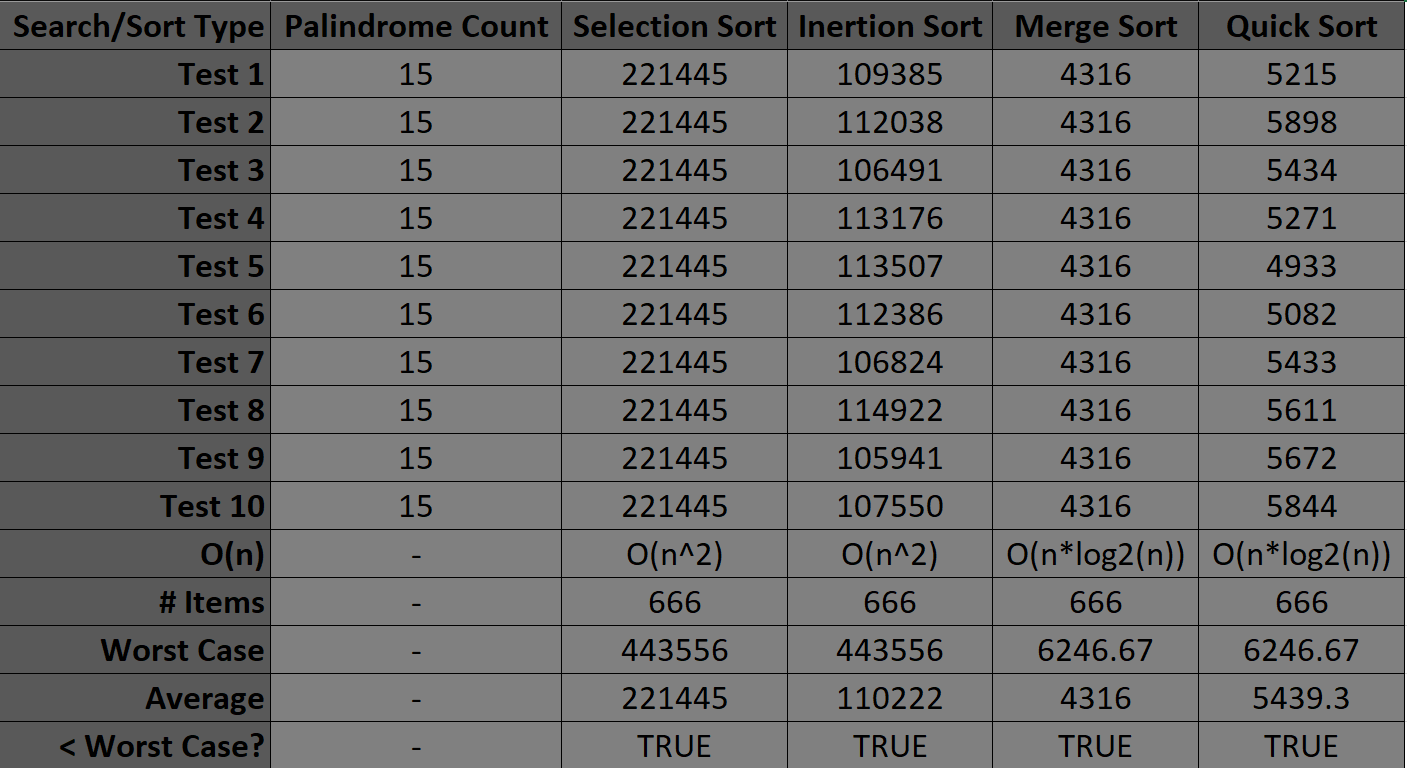
\includegraphics[width=120mm,scale=0.5]{Results.png}
\end{center}
As we can see, after running 10 tests on our data, some patterns have immerged. Firstly, notice that the number of comparisons made during the Selection and Merge Sorts. It remains the same for each test. This is because
the implementation of these sorts do not depend on how partially sorted our data is, where as Insertion and Quick sort do. Secondly, the section half of this table calculates the estimated worse case number of comparisons for
the given sort. As I have demonstrated using Excel, my sorts are all well below the expected worse case. 

\section{Prerequisites} \label{Prereq}
These are the modules and the namespace I have used for this assignment. A more detailed list of the include statements can be found on main.cpp
\lstinputlisting[language=C++, firstline=12, lastline=19]{main.cpp}
\lstinputlisting[language=C++, firstline=166, lastline=167]{main.cpp}


\section{Main} \label{Main}
The Main method of this document houses the function calls for each part of Assignment 1. As we saw in Assignment Results (Sec \ref{AssignmentResult}),
we first call the calcPalindrome() method (Sec \ref{Palindromes}) which calculates then number of palindromes in magicItems. Then the globally scoped numComparisons
is set to 0 to ensure an accurate count. Next we call the shuffleItems() method (Sec \ref{Shuffle}) which runs the Knuth Shuffle over the list of magic items and then the selectionSort() function (Sec \ref{Selection}).
As shown in the code below, the order of setting numComparisons to 0, shuffling the items, and sorting is repeated throughout Main. However, it's important to note some distinctions. After the
insertionSort() method (Sec \ref{Insertion}) is called we clear the lines vector (Ln 13/19). This is done so that a freshly shuffled deck of items is given to the sorts. 
This is only done for mergeSort() and quickSort() (Sec \ref{Merge}, \ref{Quick}) because they use recursion. So the first time they're ran, we have to give an empty vector, fill it with the shuffled items, and sort it.
Also note that since recursion is used for these sorts, we cannot have the sort itself return the number of comparisons made, we have to return it outside the function. 
\lstinputlisting[language=C++, firstline=342, lastline=369]{main.cpp}

\section{Node} \label{Node}
First I created instances of a Node class which extends a Stack(Sec \ref{Stack}) and a Queue (Sec \ref{Queue}).
This node class is comprised of a data portion which is a string (Ln 4), and a next pointer to reference the next node in order (Ln 4/10).
The method creates a node (Ln 7) with an input of some string "item" which data is set to (Ln 7/9), then the next pointer is set to NULL (Ln 10).
\lstinputlisting[language=C++, firstline=21, lastline=32]{main.cpp}

\section{Stack} \label{Stack}
Then I made a Stack class which extended the Node (Sec \ref{Node}) class. The stack has a pointer to its first element (Ln 4) called top which when a stack is made is set to NULL (Ln 9). I next implemented push(), pop(),
and isEmpty() methods to the stack (Ln 12, 19, 30). These all work how one might expect, push takes a string and makes it the new top, setting the old top to the new ones next. Pop takes the top element, returns the data, sets the
tops next to the new top, and deletes the old top. And isEmpty checks if the stack is empty and returns True if.
\lstinputlisting[language=C++, firstline=34, lastline=67]{main.cpp}

\section{Queue} \label{Queue}
Next I made a Queue class also extending the Node (Sec \ref{Node}) class. The queue has pointers to both its head and tail (Ln 4/5). When the queue is made these are set to NULL (Ln 10/11). Then, like the stack, I define methods for
enqueueing, dequeueing, and checking to see if the queue isEmpty. The enqueue() method (Ln 14) takes in a string and sets it to the head and tail if the queue is empty or sets it to the new tail if not empty (Ln 18-26). The dequeue() method (Ln 29)
is the same as the pop() method in the Stack (Sec \ref{Stack}). It returns the data of the removed element, however with queues, elements are removed from the front, so the head is dequeued, not the tail. The isEmpty() method is also the same (Ln 39).
\lstinputlisting[language=C++, firstline=69, lastline=111]{main.cpp}

\section{Palindromes} \label{Palindromes}
We are asked to calculate the number of palindromic strings there were in a given list of 666 magic items. After running the search through the vector of strings, and entering each item into a Stack (Sec \ref{Stack}) and Queue (Sec \ref{Queue}). 
Then comparing popping and dequeueing each element of the item, comparing for equality, and if equal then checking the next element. Until, if all are true then the item is a palindrome else go to next element.
We then find that the number of palindromes in the magicItems.txt file is 15. 
\lstinputlisting[language=C++, firstline=113, lastline=164]{main.cpp}

\section{List Shuffle} \label{Shuffle}
Here we define the shuffling method which is used to randomize the magicItems vector before each sort. 
This is called the Knuth sort, where we take a random index in the vector and swap the first item and that random item. Do this for each element in the vector.
\lstinputlisting[language=C++, firstline=169, lastline=191]{main.cpp}

\section{Selectio nSort} \label{Selection}
Now we move to the first of our sorting methods. The Selection sort which goes through our randomized vector, takes the first element and looks for an element less than itself. Once it has looked through the whole vector, it then swaps the
current and the lowest items, then it goes onto the next items until it reaches the end of the list, sorting it.
\lstinputlisting[language=C++, firstline=193, lastline=214]{main.cpp}

\section{Insertion Sort} \label{Insertion}
The second sorting method was Insertion sort which takes the list and compares each element one by one. Meaning the first element is compared to the second, if its greater than the second, swap, then go to the third element, if its less 
than the second swap, if its less than the first, swap again. This continues until the array is sorted
\lstinputlisting[language=C++, firstline=216, lastline=233]{main.cpp}

\section{Merge Sort} \label{Merge}
Merge sort is the first sort in this assignment to use recursion. Recursion is the best! Why? Because it recurs. Unlike the above sorts, merge sort takes in a vector of strings called list (Ln 1). When this function is called from the Main method,
it is given the list shuffled from before (Sec \ref{Shuffle}). However, when the sort recurs, it then uses a broken-up version of the original vector. Merge sort works by taking the original list, and breaking it down into halves over and over again until
each half is of length one, then it will rejoin each half, but just before it will compare if the left half is greater or less than the right half and combine accordingly to make a sorted list. Divide 'n Conquer.
\lstinputlisting[language=C++, firstline=235, lastline=294]{main.cpp}

\section{Quick Sort} \label{Quick}
Our final sort was Quick sort. Similarly to the mergeSort() method (Sec \ref{Merge}), quick sort also uses recursion to sort the magic items. However, instead of splitting the vector down the middle, we now take a random value called the partition point, 
and use that to split the vector. Everything larger then the partition point to the right and everything lower to the left. Then quick sort recurs on these smaller left and right portion, similarly to mergeSort() (Sec \ref{Merge}) until sorted. 
\lstinputlisting[language=C++, firstline=296, lastline=340]{main.cpp}

\section{Final Thoughts} \label{Final}
This assignment was a large challenge in the beginning. I am new to C++ completely and I have been using YouTube, StackOverflow, and tons of other sources to put this assignment together. It was very fun learning how to implement 
these ideas which I use in other languages in a new one. I hope all code compiles and runs flawlessly but please report any issues, I will fix them. 
\end{document}
